Es esta sección se implementará un SR-Latch y un Flip Flop D utilizando compuertas.

\subsection{SR-Latch}

Un Latch-SR es un elemento de memoria asincrónico con dos inputs (S y R), también conocido con Set-Reset Latch. A este circuito le corresponde la siguiente tabla de verdad:
\begin{table}[H]
\centering
\begin{tabular}{
>{\columncolor[HTML]{FFFFFF}}c 
>{\columncolor[HTML]{FFFFFF}}c |
>{\columncolor[HTML]{FFFFFF}}c }
\textbf{$S$} & \textbf{$R$} & \textbf{$Q_n$} \\ \hline
0            & 0            & $Q_{n-1}$      \\
0            & 1            & 0              \\
1            & 0            & 1              \\
1            & 1            & 0             
\end{tabular}
\end{table}

Se propusieron dos circuitos de implementación, utilizando para el primero compuertas del tipo NOR, mientras que para el segundo de tipo NAND, con la intención de no solo comparar los observables de interés con un modelo comercial, sino también entre distintas tipos de compuertas. Siendo los siguientes circuitos\footnote{Brown, S. and Vranesic, Z. (2002). Fundamentals of digital logic with VHDL design. 3rd ed. pp.250-251.}:

\begin{figure}[H]
\begin{center}
\begin{subfigure}{.3\textwidth}
\begin{circuitikz}
	\node [american nor port](O1){};
	\draw (O1) to[open] ++(0,-3) node[american nor port](O2){};
	\draw (O1.in 1) to[short] ++(-1,0) node[circ, label=left:$R$](R){};
	\draw (O2.in 2) to[short] ++(-1,0) node[circ, label=left:$S$](S){};

	\draw (O1.in 2) to[short] ++(0,-0.5) node[](aux1){};
	\draw (O2.in 1) to[short] ++(0,0.5) node[](aux2){};

	\draw (O1.out) to[short] ++(0,-0.75) to[short] (aux2);
	\draw (O2.out) to[short] ++(0,0.75) to[short] (aux1);
		
	\draw (O1.out) to[short] ++(1,0) node[circ, label=right:$Q$](Q){};
	\draw (O2.out) to[short] ++(1,0) node[circ, label=right:$\bar{Q}$](Qn){};
\end{circuitikz}
\end{subfigure}
\begin{subfigure}{.3\textwidth}
\begin{circuitikz}
	\node [american nand port](O1){};
	\draw (O1) to[open] ++(0,-3) node[american nand port](O2){};
	\draw (O1.in 1) to[short] ++(-1,0) node[](R){};
	\draw (O2.in 2) to[short] ++(-1,0) node[](S){};

	\draw (O1.in 2) to[short] ++(0,-0.5) node[](aux1){};
	\draw (O2.in 1) to[short] ++(0,0.5) node[](aux2){};

	\draw (O1.out) to[short] ++(0,-0.75) to[short] (aux2);
	\draw (O2.out) to[short] ++(0,0.75) to[short] (aux1);
		
	\draw (O1.out) to[short] ++(1,0) node[circ, label=right:$Q$](Q){};
	\draw (O2.out) to[short] ++(1,0) node[circ, label=right:$\bar{Q}$](Qn){};
	
	\draw (R) node[american nand port, anchor=out](A3){};
	\draw (S) node[american nand port, anchor=out](A4){};
	\draw (A3.in 2) to[short, circ] (A3.in 1) to[short] ++(-0.5,0) node[circ, label=left:$D$](){};
	\draw (A4.in 1) to[short, circ] (A4.in 2) to[short] ++(-0.5,0) node[circ, label=left:$S$](){};
\end{circuitikz}
\end{subfigure}
\caption{Circuito Propuesto SR-Latch.}
\label{fig:circsrlatch}
\end{center}
\end{figure}

Se lleva a cabo utilizando compuertas NOR y NAND, se eligió el integrado \href{https://pdf1.alldatasheet.com/datasheet-pdf/view/228632/ONSEMI/74HC02.html}{74HC02} debido a que es High-Speed y ya que no es necesario compatibilidad con TTL, como se analizó en el punto (2). 

Se toman como observables de interés el tiempo de propagación:
\begin{equation*}
\begin{split}
	t_{p-SQ}: S \implies Q \\
	t_{p-RQ}: R \implies Q
\end{split}
\end{equation*}

Estos tiempos son comparados con un integrado \href{http://noel.feld.cvut.cz/hw/st/1937.pdf}{74HC279}, el cual contiene 4 SR-Latch. Las mediciones hechas se ven en la siguiente tabla:
\begin{table}[H]
\centering
\begin{tabular}{cccl}
\hline
\textit{}           & \textbf{Circuito NOR} & \textbf{Circuito NAND} & \textbf{74HC279} \\ \hline
\textbf{$t_{p-RQ}$} & 8.3nS                 & 43.2ns                 & 8nS              \\
\textbf{$t_{t-RQ}$} & 4.83nS                & 4nS                    & 14nS             \\
\textbf{$t_{p-SQ}$} & 24.24nS               & 18ns                   & 15nS             \\
\textbf{$t_{t-SQ}$} & 11nS                  & 4ns                    & 8nS             \\
\hline
\end{tabular}
\end{table}

Es notable que los tiempos son similares. Por otro lado, el espacio que ocupan no lo es, dado que toma el doble de integrados para la misma cantidad de Latches.
 
\subsection{Flip Flop D}

Un Flip Flop D es un elemento de memoria sincrónico, el cual cuenta con 2 entradas, siendo una de clock y la otra de la información (Data). Le corresponde la siguiente tabla de verdad:
% Please add the following required packages to your document preamble:
% \usepackage[table,xcdraw]{xcolor}
% If you use beamer only pass "xcolor=table" option, i.e. \documentclass[xcolor=table]{beamer}
\begin{table}[H]
\centering
\begin{tabular}{
>{\columncolor[HTML]{FFFFFF}}c 
>{\columncolor[HTML]{FFFFFF}}c |
>{\columncolor[HTML]{FFFFFF}}c }
\hline
\textbf{Clock} & \textbf{$D$} & \textbf{$Q_n$} \\ \hline
$\downarrow$   & X            & $Q_{n-1}$      \\
$\uparrow$     & 0            & 0              \\
$\uparrow$     & 1            & 1             \\
\hline
\end{tabular}
\end{table}

El circuito de implementación propuesto es el siguiente\footnote{Brown, S. and Vranesic, Z. (2002). Fundamentals of digital logic with VHDL design. 3rd ed. pp.254-256.}:

\begin{figure}[H]
\begin{center}
\begin{circuitikz}

	\node [american nand port](O1){};
	\draw (O1) to[open] ++(0,-3) node[american nand port](O2){};
	\draw (O1.in 1) to[short] ++(-1,0) node[](R){};
	\draw (O2.in 2) to[short] ++(-1,0) node[](S){};

	\draw (O1.in 2) to[short] ++(0,-0.5) node[](aux1){};
	\draw (O2.in 1) to[short] ++(0,0.5) node[](aux2){};

	\draw (O1.out) to[short] ++(0,-0.75) to[short] (aux2);
	\draw (O2.out) to[short] ++(0,0.75) to[short] (aux1);
		
	\draw (O1.out) to[short] ++(1,0) node[circ, label=right:$Q$](Q){};
	\draw (O2.out) to[short] ++(1,0) node[circ, label=right:$\bar{Q}$](Qn){};
	
	\draw (R) node[american nand port, anchor=out](A3){};
	\draw (S) node[american nand port, anchor=out](A4){};
	\draw (A3.in 2) -- (A4.in 1);
	
	\draw (A3.in 2) to[open] ++(0,-1.5) to[short] ++ (-2,0) node[circ, label=left:$Clk$](){};
	
	\draw (A3.in 1) node[label=north:$S$](){};
	\draw (A3.in 1) to[short] ++(-2,0) node[circ, label=north:$D$](D){};
	
	\draw (A4.in 2) node[label=north:$R$](){};
	\draw (A4.bin 2) node[ocirc](){};
	\draw (A4.in 2) to[short] ++(-1,0) node[](aux3){};
	
	\draw (D) to[open] ++(1,0) to[short] (aux3);
\end{circuitikz}
\caption{Circuito Propuesto Flip Flop D.}
\label{fig:circsrlatch}
\end{center}
\end{figure}

Este circuito se lleva a cabo utilizando compuertas NAND. Se eligió el integrado \href{https://pdf1.alldatasheet.com/datasheet-pdf/view/351460/ONSEMI/74HC132.html}{74HC132} debido a que es High-Speed y no es necesaria la compatibilidad con TTL, como se analizó en el punto (2). También para el clock se realizó un Edge-Detector implementado con el circuito presentado a continuación. Este dispositivo es anexado al circuito implementado con NANDS del latch SR.
\begin{figure}[H]	
	\centering
	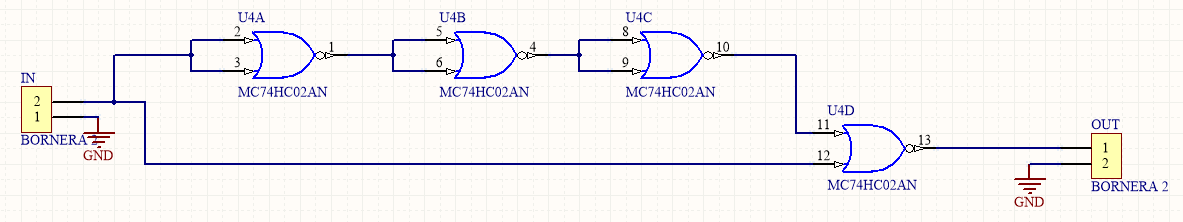
\includegraphics[width=0.8\textwidth]{ImagenesEjercicio6/edgedetector.PNG}
	\caption{Edge-Detector realizado.}
	\label{fig:circedge}
\end{figure}

Se toman como observables de interés el tiempo de propagación y de transición:
\begin{equation*}
\begin{split}
	t_{p-DQ}: D \implies Q \\
	t_{t-DQ}: Q=0 \implies Q = 1
\end{split}
\end{equation*}
 
En cuanto a la medición de estos tiempos, se tuvo la problemática de que el rise time de las compuertas eran menores que el rise time del osciloscopio. Para algunas de ellas se logró conseguir uno con mayor ancho de banda, lo cual mejoró las mediciones.

Estos tiempos medidos son comparados con un integrado \href{https://pdf1.alldatasheet.com/datasheet-pdf/view/15593/PHILIPS/74HC374.html}{74HC374}, el cual contiene 8 Flip Flop D. Las mediciones hechas se ven en la siguiente tabla:
\begin{table}[H]
\centering
\begin{tabular}{ccc}
\hline
\textit{}                               & \textbf{Circuito}         & \textbf{74HC374}     \\ \hline
\textbf{$t_{p-DQ}$}                     & 23.6nS                    & 16nS                 \\
\textbf{$t_{t-DQ}$}                     & 4.43nS                    & 5nS                  \\
\hline
\end{tabular}
\end{table}